\section{Serge Haroche}
One half of the Nobel prize in physics 2012 was awarded to the french quantum
physicist Serge Haroche. Serge Haroches main work concentrates on the field of
cavity quantum eledtrodynamics (CQED), i.e. in his case the interaction of
Rydberg atoms with single modes in a cavity. In this section we will follow some
of the steps of his personal life and scientific carreer in order to understand how he
made his way to the Nobel prize. 

\subsection{Early Life and Scientific Carreer}
\begin{wrapfigure}{r}{0.33\textwidth}
  \centering
  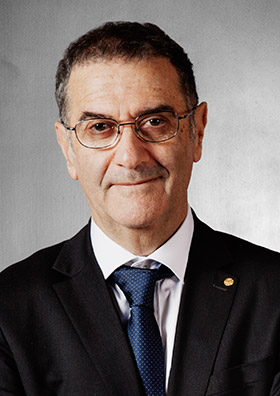
\includegraphics[width=.2\textwidth]{haroche.jpg}
  \caption{Serge Haroche in 2012.\\ Source: \textit{nobelprize.org}}
\end{wrapfigure}
Serge Haroche was born 11 September 1944 in Casablanca, a major city at the
moroccon atlantic coast, as the son of Albert and
Valentine Haroche, both teachers at a local jewish school. At that time the
southern part of Morocco was a French protectorate. However in 1956 Morocco
gained independence and Haroches parents moved to Paris as they felt that they
had themselves received and given their children a french education. Regarding
his performance in school, Haroche seemed to have no problem settling in, as he
was ``immediately at the head of [his] class''~\cite{shbio} at his new school in
Paris. After his ``Baccalauréat''\footnote{The french correspondence to the german
``Abitur''.} he joined the for two years of continuous training and examination to
eventually be admitted to one of the french elite universities. Being the best
of his year in the national ranking, he was able to join ``École normale
supérieure''(ENS) in 1963 where he studied until 1967 and was taught, among
others, by Alfred Kastler\footnote{Nobel prize for physics in 1966 ``for the
development of optical methods for studying Hertzian resonances in atoms''.} and
Claude Cohen-Tannoudji.\footnote{Nobel prize for physics in 1997 ``for the
development of methods to cool and trap atoms with laser light''.} At the end of
his studies he was ``enthralled by the mysterious beauty of the quantum
world''~\cite{shbio} and decided to continue his academic carreer in the field of
quantum physics, more specifically quantum optics. He decided to write a PhD
thesis with Cohen-Tannoudji as his supervisor on the dressed states
formalism (see
Sec.~\ref{sec:DressedStates}) and its implications on the description of
optically pumped atoms. In the experiments he performed, he used spectral lamps
as a light source but it became clear for him that he needed to learn how to
apply lasers to his field of research.

After his PhD at ENS, Serge Haroche joined the group of Arthur
  Schawlow\footnote{Nobel prize for physics in 1981 ``for his contribution to
  the development of laser spectroscopy''. } at
Stanford University from 1972 to 1973. Shortly before is arrival Theodor
Hänsch\footnote{Nobel prize for physics in 2005 ``for his contribution to the
development of laser-based precision spectroscopy''.}
had joined the group as an associate professor, making him the fourth later
Nobel laureate to work with Haroche. Schawlow gave a lab room and a pulsed dye
laser to Haroche and told him that ``it was up to [him] to find something
interesting to do with it''~\cite{shbio}. As Haroche was already familiar with
the dressed states formalism and saw the potential of the laser as a much more
intense light source compared to classical lamps, he decided to probe
quantum beat signals in  cesium vapor~\cite{haroche1973hyperfine}. The resulting
paper will be discussed in Sec.~\ref{sec:QuantumBeats}. Still in Stanford
Haroche sent a research proposal on the study of Rydberg atoms to one of the ENS
directors and was immediately offered a position and start-up budget. His own
research in the labs of ENS started in 1973 and has continued ever since with
Rydberg atoms being a central pillar of many experiments.\footnote{See for example
\cite{haroche1983EnhancedSpontEm,haroche1990QND,haroche1999SinglePhoton,haroche2007QuantumJumps}}
At ENS Haroche had a position as ``maître de recherche'' that allowed him to
fully focus on his research. However he was also keen to teach students, what
drove him to take on a position as a full professor of physics at Université
Paris VI. In the early 1980s Haroche started his research in the field of cavity
quantum electrodynamics (CQED) on which all of his later explorations of
fundamental quantum mechanical concepts are based. His research on CQED will be
adressed with the discussion of some exemplary experiments in
Sec.~\ref{sec:CQED}. At this time Haroche already had a good reputation as a
scietist and was offered a position in Harvard in 1981 which he refused. When he
was tempted again in 1984, this time by the University of Yale, he accepted and
was appointed a professor while at the same time retaining his position in
Paris. He kept the chair in Yale until 1993 and during this time was able to run
succesful experiments on both sides of the atlantic
\cite{haroche1983EnhancedSpontEm, haroche1987SupressedEmission}. In 2001 Haroche
was appointed professor of quantum physics at Collège de
France~\cite{harocheCollege}. The Collège de France is a prestigious institution
at which scientists from different fields give lectures on their current
research that are open to the public. In 2009 Haroche was awarded the gold medal
of the Centre national de la récherche scientifique, one of the highest honors
awarded to french scientists once a year.

\subsection{Quantum Beats}
\label{sec:QuantumBeats}
During his Postdoc in Stanford Haroche investigated the phenomenon of quantum
beats that appear in the fluorescence intensity in some types of atoms when they
are excited to a superposition of upper states and decay towards a common lower
lying state~\cite{haroche1973hyperfine}. Quantum beats where especially interesting as they could only be
entirely described by quantum electrodynamics (QED), i.e. in a model in which
not only the energy levels of the atom but also the states of the light field
are quantized.


\begin{figure}[t]
  \centering
  \begin{subfigure}[t]{0.4\linewidth}
    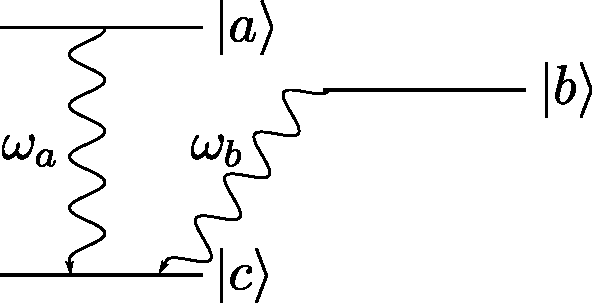
\includegraphics[width=\linewidth]{v_type_atom.pdf}
    \caption{V-type atom}
    \label{fig:V_type}
  \end{subfigure}
  ~
  \begin{subfigure}[t]{0.4\linewidth}
    \centering
    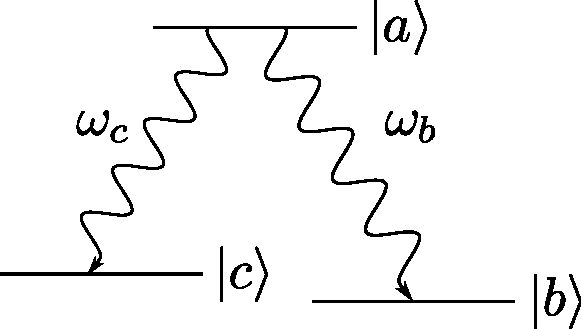
\includegraphics[width=\linewidth]{lambda_type_atom.pdf}
    \caption{$\Lambda$-type atom}
    \label{fig:lam_type}
  \end{subfigure}
  \caption{Atom level schemes for which there should be quantum beat signals in the
    emmitted intensity in a semi-classical model. In QED only (a) shows quantum
beats which is in accordance with experiment.}
  \label{fig:atom_types}
\end{figure}

The two types of atoms that are interesting with regards to quantum beats are
shown in Fig.~\ref{fig:atom_types}. V-type atoms have two upper levels $\ket{a}$
and $\ket{b}$ that can decay to a common lower lying state $\ket{c}$ but
transitions between them are dipole forbidden. $\Lambda$-type atoms consist of
one upper level $\ket{a}$ that can decay to two different lower lying levels
$\ket{b}$ and $\ket{c}$. Summarizing the QED calculations in
\cite{scully1997QuantumBeats}, for V-type atoms one expects a modulation on top
of the intensity signal of the form
\begin{align}
  \label{eq:quantum_beat}
  I_{tot}(t) = I_0 + I_{\text{beat}} \cos\left\lbrace \left(\omega_a -
  \omega_b\right) t\right\rbrace
\end{align}
whereas for $\Lambda$-type atoms, the beat term vanishes. This result is in
disagreement with a semiclassical approach in which both types show a beat term.
However only the QED results are consistent with performed experiments.

\begin{figure}[t]
  \centering
  \begin{subfigure}[t]{0.48\linewidth}
    \centering
    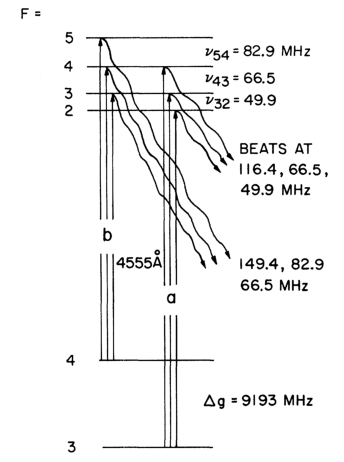
\includegraphics[width=.8\linewidth]{SH_quantum_beats_plot.pdf}
    \caption{Level scheme of the Cesium hyperfine structure. Pulsed excitation
    from either of the lower levels (F=3,4) introduces the two possible sets of
  quantum beats $a$ and $b$ with beat frequencies indicated.}
    \label{fig:cs_level_scheme}
  \end{subfigure}
  ~
  \begin{subfigure}[t]{0.48\linewidth}
    \centering
    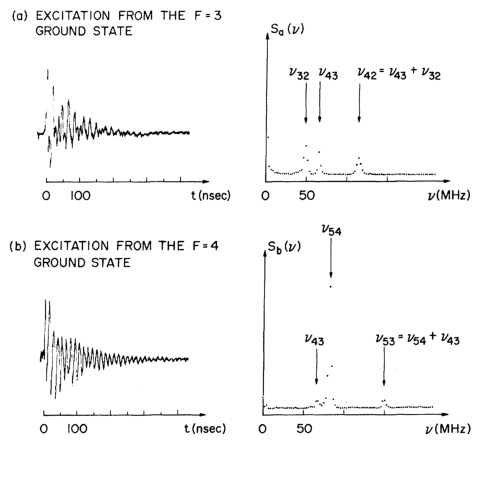
\includegraphics[width=\linewidth]{SH_quantum_beats_results_ws.pdf}
    \caption{Recorded intensities (left) and Fourier analysis (right) for the
    two different types of excitation. The frequency spectrum exhibits
  characteristic maxima in both cases.}
    \label{fig:cs_beat_results}
  \end{subfigure}
  \caption{Hyperfine structure of cesium and experimentally measured
    fluorescence intensities, showing a
     quantum beat signal as predicted by
  QED.(Source:~\cite{haroche1973hyperfine})}
  \label{fig:quantum_beats_experiment}
\end{figure}

The system of interest for Serge Haroche was the Cesium hyperfine structure
shown in Fig.~\ref{fig:cs_level_scheme}. The frequency bandwidth of the pulsed
dye laser is smaller than the splitting of the two lower levels, but large
enough to populate all possible upper states. This means that e.g. from the F=3
ground state, the F$^\prime$=2,3,4 excited states can be populated according to
the dipole selection rule. In this way two sets of upper states can be excited,
namely $a$ and $b$ in Fig~\ref{fig:cs_level_scheme}. The expected beat
frequencies are the three difference frequencies between the upper levels.

The experimental results are shown in Fig~\ref{fig:cs_beat_results}. The
fluorescence intensities on the left show a clear oscillating behaviour, with an
exponentially decaying enveloppe caused by the characteristic damping of
spontaneous emission. The plots on the right show the Fourier spectrum of the
intensity signals. In each off them there are three characteristic peaks that
correspond to the three beat frequencies indicated in
Fig.~\ref{fig:cs_level_scheme}. 

The resulting frequencies were in good agreement with other values that had been
measured for the hyperfine structure of cesium. Although the uncertainties were
higher than those of other state of the art spectroscopy methods there was a
clear advantage of this method: once one is able to excite the upper states,
there is no need to scan for resonance as the full intensity spectrum already
exhibits the needed modulation. A very finely tunable laser is thus not
necessary. Further, the precision of the method could be improved by increasing
the sampling frequency and the total number of sample points taken.


\subsection{Cavity Quantum Electrodynamics}
\label{sec:CQED}
After his first experiments in quantum optics, Serge Haroche soon turned towards
his very own field of research: cavity quantum electrodynamics (CQED). CQED
deals with the interaction of light that is confined in a cavity with atoms
e.g. passing through it. The cavity can be used to engineer coherent photon number
states $\ket{n}$ with $n$ going down to 0 or 1. In this regime the quantum
nature of light can be revealed. The following section will go through some of
the experiments performed by Haroche that revealed or made use of the quantum
behaviour of photons. 

\subsubsection{Enhanced spontaneous Emission}
\label{sec:EnhancedSpontEm}

\begin{figure}[t]
  \centering
  \begin{subfigure}[t]{0.48\linewidth}
    \centering
    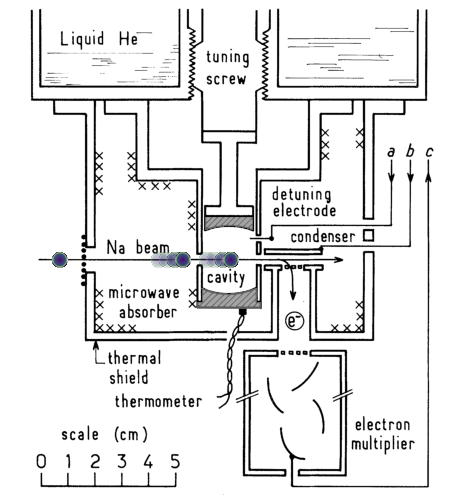
\includegraphics[width=.9\linewidth]{SH_cavity_enhanced_em_setup_rep.pdf}
    \caption{The superconducting cavity in the center can be tuned using a screw
    and is cooled by liquid helium. After crossing the cavity, the atoms states
  are detected in the ionization detector.}
    \label{fig:cavity_enhanced_setup}
  \end{subfigure}
  ~
  \begin{subfigure}[t]{0.48\linewidth}
    \centering
    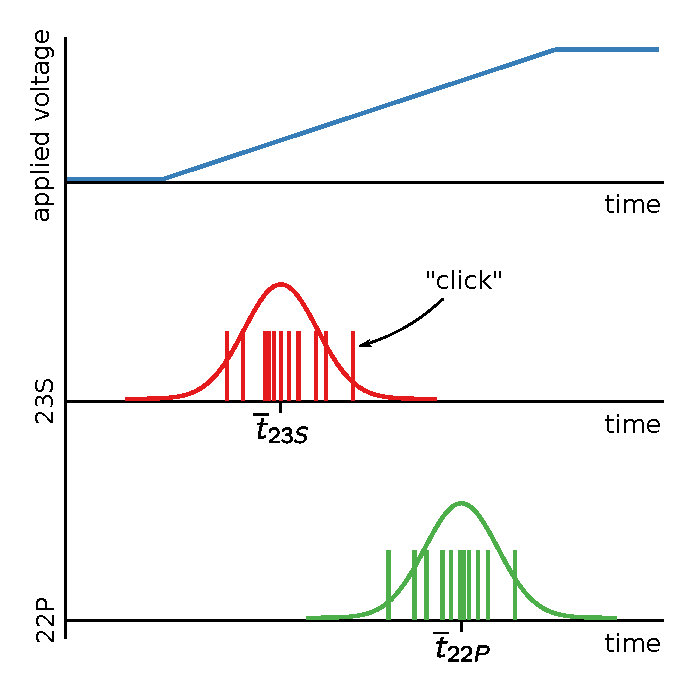
\includegraphics[width=.9\linewidth]{SH_ionization_detection_rep.pdf}
    \caption{The voltage applied to the condenser is increased in time. The
    different ionization energies of the 23S and the 22P states lead to
  different electron detection times in the electron multiplier.}
    \label{fig:ionization_detection}
  \end{subfigure}
  \caption{Experimental setup and ionization detection scheme used to observe
  cavity enhanced spontaneous emission. (Adapted
from~\cite{haroche1983EnhancedSpontEm})}
  \label{}
\end{figure}

One of the first experiments of the ENS group of Haroche investigated the effect
of enhanced spontaneous emission rates of an excited atom flying through a
resonant cavity~\cite{haroche1983EnhancedSpontEm}. When an atom prepared in
the upper of two levels, seperated by $\hbar \omega=\frac{h\lambda}{c}$, is brought into a cavity
that is tuned to resonance with $\omega$, the spontaneous emission rate will
be increased as
\begin{align}
  \label{eq:enh_spont_em_rate}
  \Gamma_{\text{cav}} = \Gamma_0 \frac{3Q\lambda^3}{4\pi^2 V} \equiv
  \Gamma_0\,\eta_{\text{cav}},
\end{align}
where $\Gamma_0$ is the natural decay rate, $Q$ is the Q-value of the cavity and
$V$ its mode volume. Observations of this effect in the optical range (e.g. in
Fabry-Perot interferometers) were impossible even for very high Q-values as the
volume $V$ is typically much larger than $\lambda^3$. Rydberg atoms played a key
role in the detection, as their transitions are typically in the \Si{mm}
wavelength, an order of magnitude in which cavities can be manufactured.

The experimental setup used by Haroche et.al. is shown in
Fig~\ref{fig:cavity_enhanced_setup}. The central part is the supeconducting
niobium cavity cooled down to \SI{5.7}{K} with an estimated Q-value of the order
of $10^6$ and an effective mode volume of $V=\SI{70}{mm^3}$, surrounded by an absorbant
shielding to isolate it from background radiation. A micrometer screw allows
tuning of the cavity's resonance frequency. To detect the increased spontaneous
emission rate, sodium atoms are prepared in the 23S Rydberg state. The
23S $\rightarrow$ 22P transition has a wavelength of $\lambda=\SI{0.88}{mm}$
which makes observation of the effect possible for the given Q-value. The final
state of the atoms, after having crossed the cavity, is determined by using a
combination of a condenser and a time resolved electron detector. The detection
scheme is depicted in Fig.~\ref{fig:ionization_detection}, showing the voltage
applied to the condenser and two exemplary detection patterns in the electron
multiplier as a function of time. One exploits the feature that the 23S state
and the 22P state have different ionization energies. Ramping up the voltage
with time will thus on average result in different ionization times
corresponding to different electron detection times $\overline{t}_{23S}$ and
$\overline{t}_{22P}$. When the cavity is tuned to resonance, the share of atoms
in the 22P state should increase caused by an increase of the transition rate
$\Gamma_{23S \rightarrow 22P}$.

\begin{figure}[t]
  \centering
  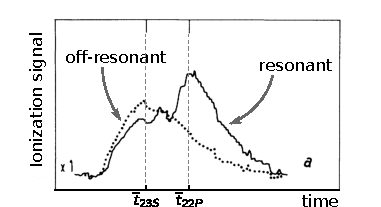
\includegraphics[width=.5\linewidth]{SH_cavity_enhanced_em_results_rep.pdf}
  \caption{Ionization signal of the atoms after crossing the cavity which is either
  off-resonant (dotted line) or resonant (solid line). An increased population
of the 22P state is observed in the resonant case.}
  \label{fig:SH_cavity_enhanced_em_results_rep}
\end{figure}
This expectation exactly matches the experimental results shown in
Fig.~\ref{fig:SH_cavity_enhanced_em_results_rep}. One sees a clear shift of the
peak in the ionization time histogram from $\overline{t}_{23S}$ to
$\overline{t}_{22P}$ when the cavity is tuned from off-resonance to resonance.
That means that tuning the cavity to resonance indeed increases the spontaneous
emission rate as predicted by the CQED result \eqref{eq:enh_spont_em_rate}.


Haroche and his group at ENS where the first to give experimental evidence of
this CQED effect. But soon others followed. Namely the group of Haroche at Yale
who were able to show that also a suppression of certain modes is possible
using a similar experiment that will be described in the following section.

\subsubsection{Supressed spontaneous Emission}
Another interesting effect that a surrounding cavity can have on the energy
states of an atom is the suppression of spontaneous emission. This effect was
first experimentally realized by Haroche and his group in Yale in
1986~\cite{haroche1987SupressedEmission}. 
\begin{figure}[h]
  \centering
  \begin{subfigure}[t]{.48\linewidth}
    \centering
    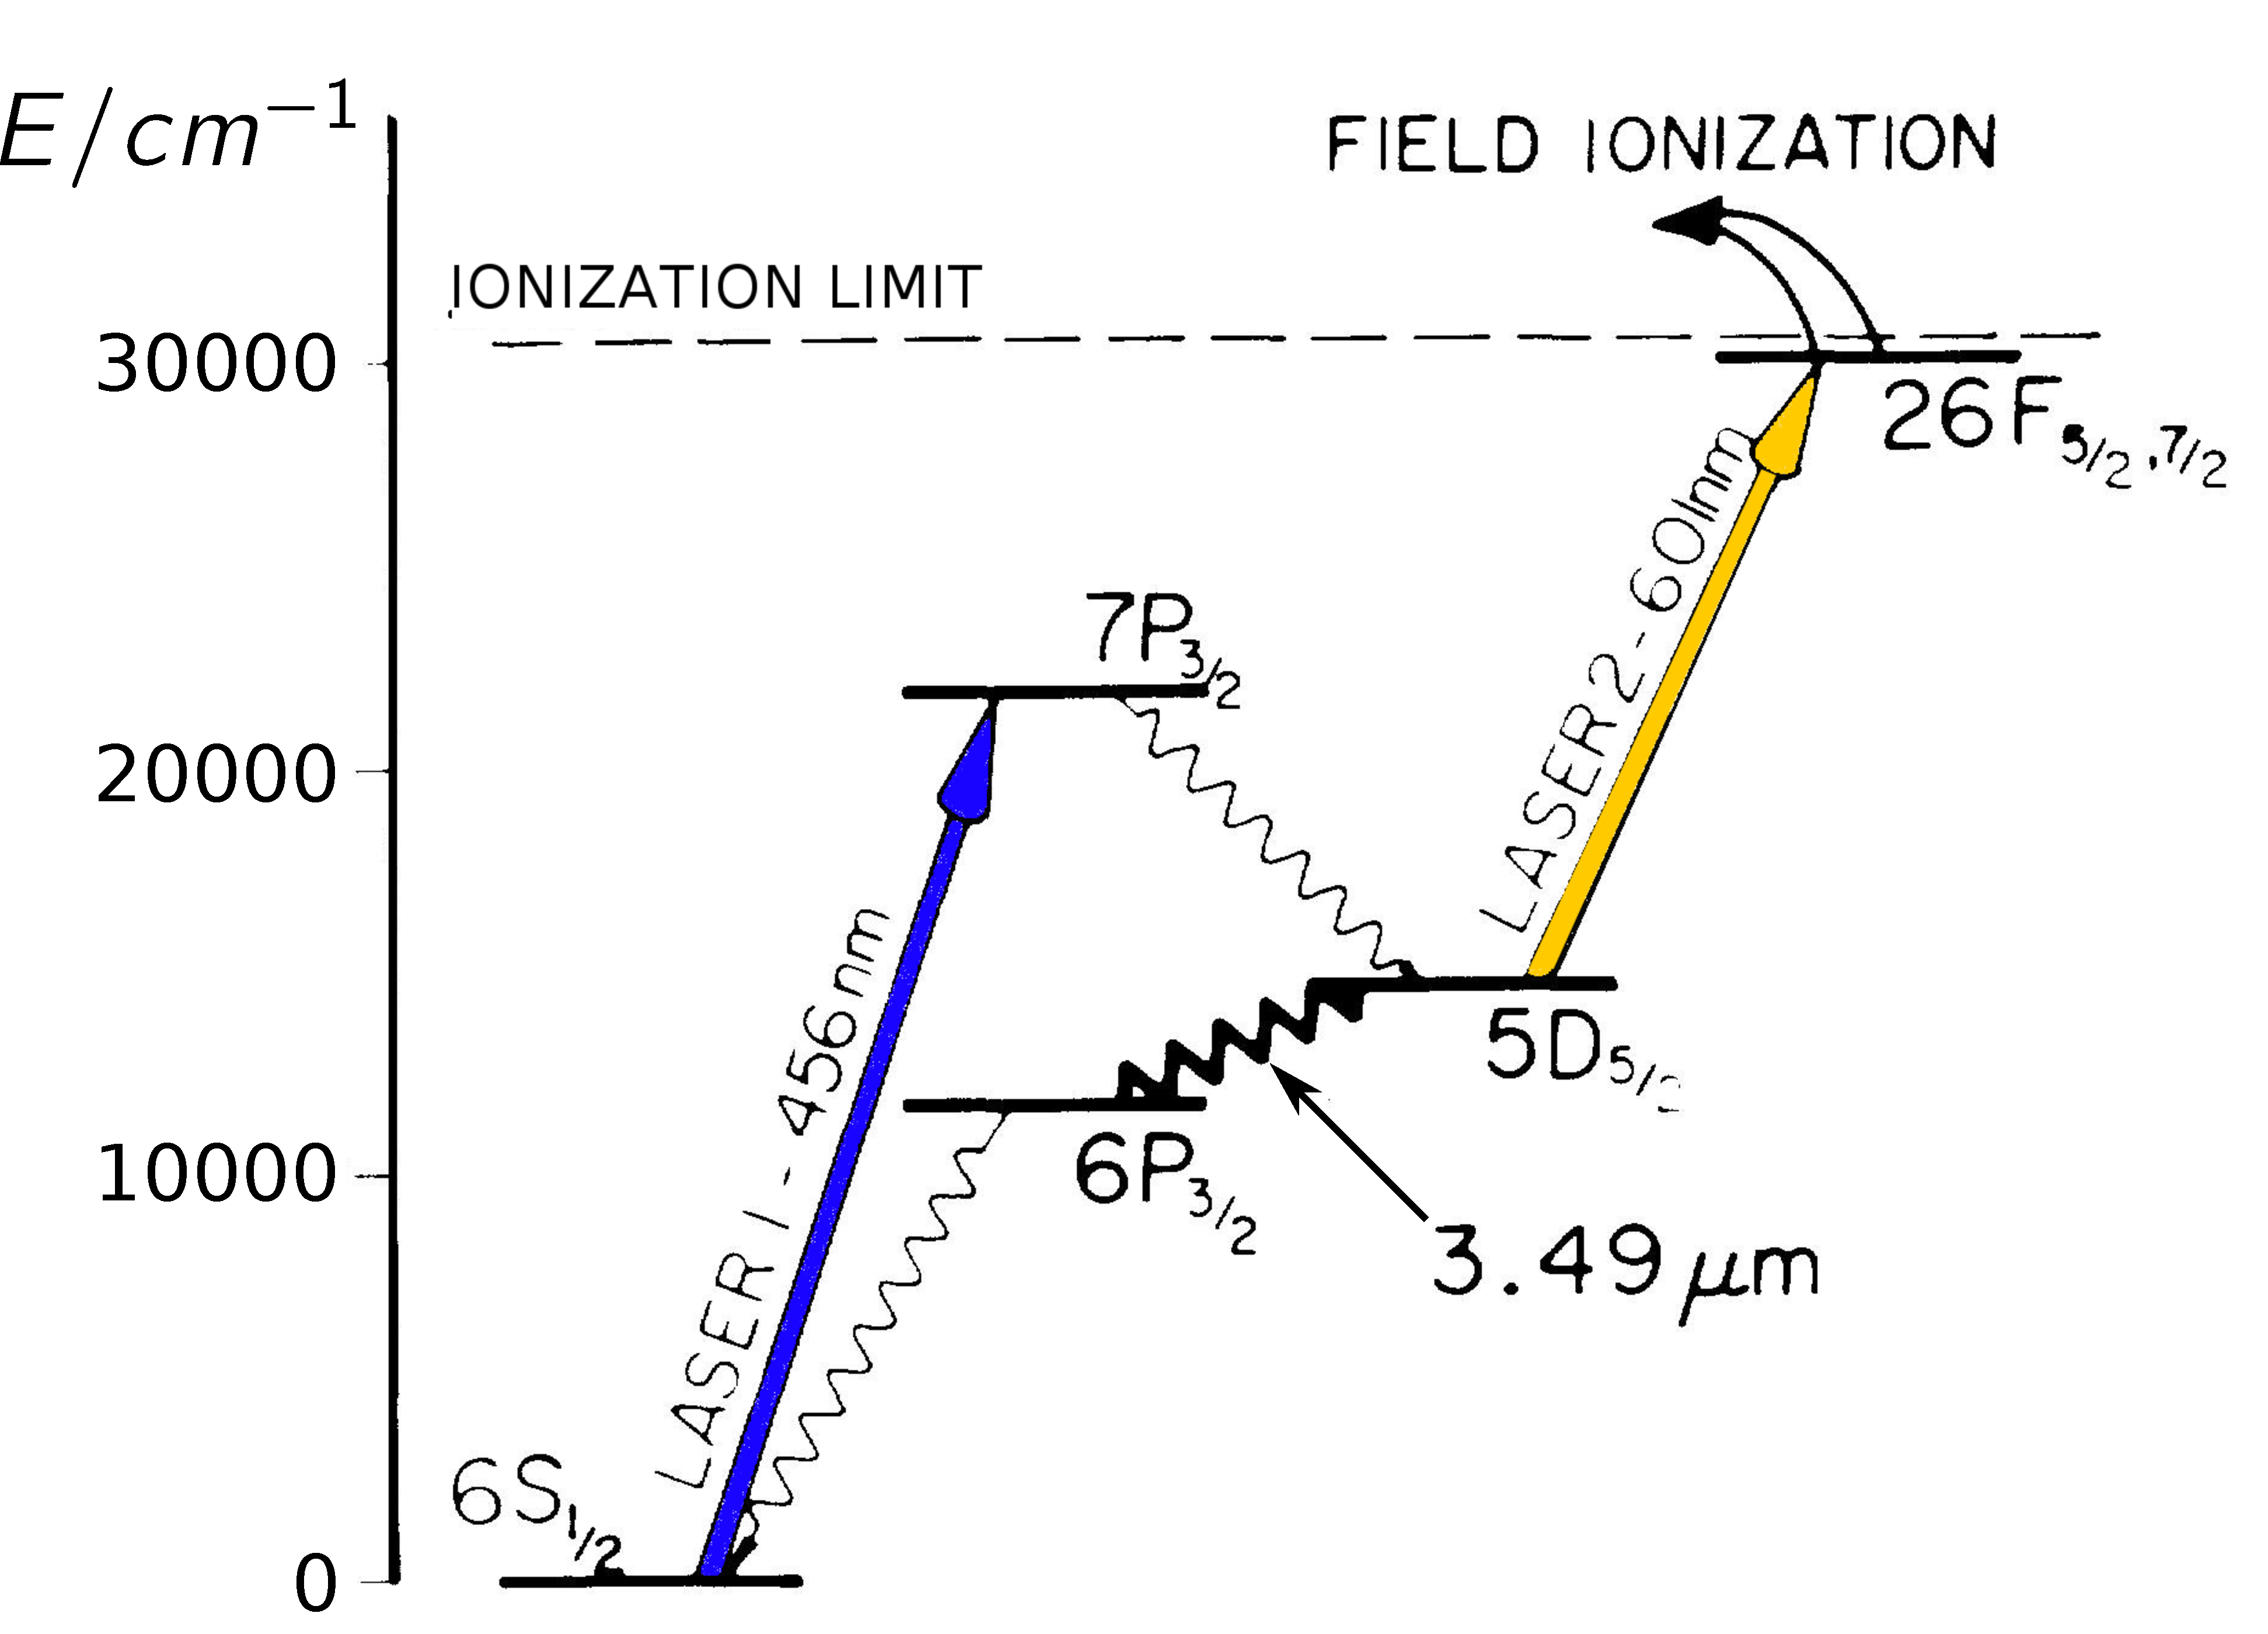
\includegraphics[width=\linewidth]{SH_supression_spont_em_scheme.pdf}
    \caption{Level scheme of the used cesium atoms. Before entering the cavity,
    the atoms are prepared in the 5D$_{5/2}$ state by excitation to 7P$_{3/2}$
    and spontaneous emission. The second laser drives the transition
  5D$_{5/2} \rightarrow 26F$.}
    \label{fig:supression_scheme1}
  \end{subfigure}
  ~
  \begin{subfigure}[t]{.48\linewidth}
    \centering
    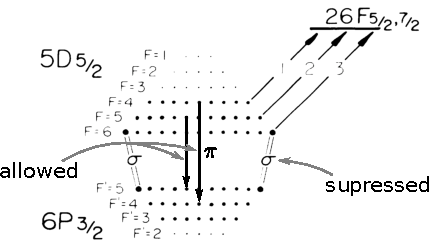
\includegraphics[width=\linewidth]{SH_supression_spont_em_scheme2.pdf}
    \caption{Hyperfine structure of the 5$D_{5/2}$ and 6P$_{3/2}$ levels. Due to
    the polarization dependend cut-off in the cavity, only $\pi$ transitions are
    allowed. The F=6 substate of 5D$_{5/2}$ can only decay via
  $\sigma$ transitions.}
  \label{fig:supression_scheme2}
  \end{subfigure}
  \caption{Relevant energy levels of cesium and their hyperfine structure. The
  different colors (blue and yellow) correspond to the two different lasers that
are used.(Source: \cite{haroche1987SupressedEmission})}
\end{figure}
When the distance between the mirrors
of the cavity $d$ becomes smaller than half the wavelength $\lambda$ of a
certain transition in the atom, i.e.
\begin{align}
  \label{eq:supress_spont_em}
  d < \frac{\lambda}{2},
\end{align}
then all transitions of this wavelength that are $\sigma$ polarized (i.e.
parallel to the mirror surface) are supressed. A pictorial explanation would be
the following: as the spontaneous emission rates depend on the vacuum
fluctuations, but the boundary conditions imposed by the mirrors do not allow
modes that fulfill \eqref{eq:supress_spont_em}, spontaneous emission for
these modes is inhibited. Nonetheless, any $\pi$ transition (polarized
perpendicular to the mirrors) is still allowed and can even be enhanced. So to
observe the anomalous survival of a state caused by a cavity, one needs to
identify a state from which only $\sigma$ decay is possible.\footnote{In
principle one could also calculate the change in the decay rate of a state
depending on the share of $\pi$ and $\sigma$ transitions, but the survival of an
else decaying state is easier to measure.}

Haroche and his group chose to use cesium atoms and identified the 5D$_{5/2}$
level to be suited for their purpose. As can be seen in the level scheme in
Fig.~\ref{fig:supression_scheme1}, the 5D$_{5/2}$ level decays to the 6P$_{3/2}$
level via emission of \SI{3.49}{\micro\meter} radiation. Looking at the
hyperfine structure of this transition  shown in
Fig.~\ref{fig:supression_scheme2} we see that the F=6 substate of
5D$_{5/2}$ can only decay via $\sigma$ emission.  


\begin{figure}[t]
  \centering
  \begin{subfigure}[t]{.48\linewidth}
    \centering
    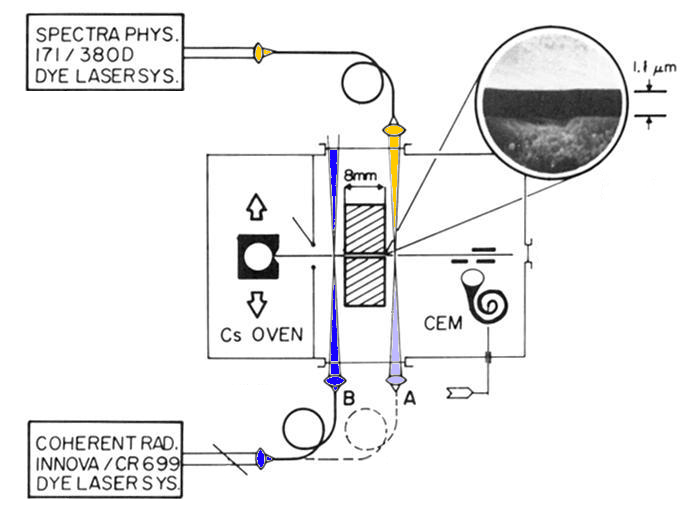
\includegraphics[width=\linewidth]{SH_supressed_spont_em_setup.jpg}
    \caption{The cavity used to cut off certain modes is \SI{1}{\micro\m}. Two
    lasers are used in cw mode, colored corresponding to the transitions shown
    in Fig.~\ref{fig:supression_scheme1}. A condenser with constant voltage
    together with a channel electron multiplier (CEM) is
    used to detect the 26F state similar to the previous experiment.}
    \label{fig:supression_setup}
  \end{subfigure}
  ~
  \begin{subfigure}[t]{.48\linewidth}
    \centering
    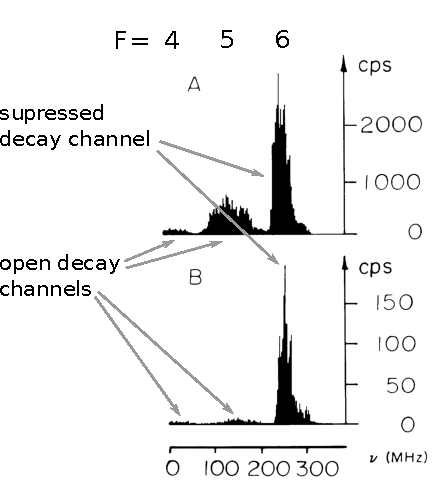
\includegraphics[width=.8\linewidth]{SH_supression_spont_em_results.pdf}
    \caption{Resulting counting rates in the CEM as a function of the frequency
      of the detection laser (yellow). Shown for atoms not having crossed (A) and having
  crossed (B) the cavity. Only atoms in the F=6 substate survive the flight
through the cavity.}
  \label{fig:supression_results}
  \end{subfigure}
  \caption{Setup and experimental results showing the supression of spontaneous
  emission of some of the transitions in the cesium hyperfine structure.
  (Adapted from \cite{haroche1987SupressedEmission})}
\end{figure}
The setup that exploits this features of cesium is shown in
Fig.~\ref{fig:supression_setup}. A directed beam of cesium atoms is leaving an
oven. First a pumping laser (blue) is used to prepare the
atoms in the 5D$_{5/2}$ state (see Fig.~\ref{fig:supression_scheme1}). Next the
atoms pass through the \SI{1.1}{\micro\meter} wide cavity, made of gold coated
fused silica blocks. A cavity of this size will supress any of the
5D$_{5/2}\rightarrow$\,6P$_{3/2}$ $\sigma$-transitions and thus supress any
transition of the F=6 substate of 5D$_{5/2}$ (see
Fig.~\ref{fig:supression_scheme2}). A \SI{240}{\micro\tesla} magnetic field
perpendicular to the mirror surfaces will align the atoms along a common axis.
After the cavity the atoms fly through the beam of the detection laser (yellow)
that can be tuned around the 5D$_{5/2}\rightarrow$\,26F transition hence
selectively pumping atoms from the hyperfine levels of 5D$_{5/2}$ to the Rydberg
state 26F. Any atom in the 26F state will then be ionized in a condenser with a
constant voltage of \SI{1}{\kilo\volt}, the ionization electron being detected
in a channel electron multiplier.

In this way (again using the properties of Rydberg atoms) the relative
populations of the several substates of 5D$_{5/2}$ can be determined. The
resulting counting rates of the CEM are shown in
Fig.~\ref{fig:supression_results}. The upper histogram shows the counting
rates depending on the resonant substate with the pumping laser placed directly before the
detection laser. This corresponds to the relative populations resulting from the
pumping process. The lower histogram shows the counting rates for the case
in which the atoms interact with the pumping laser before entering the cavity
and are pumped to the 26F by the detection laser after having traversed the
cavity. Besides the fact that the counting rates are generally lower, due to a
loss of atoms in the cavity, one sees that the peaks for the F=4 and F=5
substates of 5D$_{5/2}$ almost vanish completely compared to the peak of the F=6
substate. This is experimental evidence that the decay of F=6 is strongly
supressed by the surrounding cavity.

The preceeding experiments all show the behaviour of light as a quantum, yet the
wave function of the photon was not observed in a direct manner. This would
change with Haroches experiments on quantum non demolition measurement of
photons, which will be introduced in the next section.


\subsubsection{Quantum Non Demolition Measurement of Photons}
\label{sec:QND}
Many experiments (like the ones in the preceeding sections) show traces of the
quantum nature of photons. However ``in-vito'', i.e. non destructive,
measurement of the photons wavefunction was not performed until
2007,\footnote{For example a photodiode detects photons by absorption of the
  photon and creatin of an electron-hole pair, that
means the photons are destroyed in the detection process.} when Haroche and his
group at ENS introduced the first working experimental setup able to count an
individual photon without destroying it. To implement the quantum non demolition
(QND) measurement of photons, Haroche used many of the things he had learned
about Rydberg atoms and their interaction with light in a cavity. A proof of
concept paper about the technique had already been published in 1999~\cite{haroche1999SinglePhoton}, 
but it took Haroche and his group another seven
years to create a cavity with a Q-value so high that it could store photons with
a typical lifetime of $\tau_\gamma = \SI{0.1}{\second}$~\cite{kuhr2006ultrahigh}. 
In this cavity thermal photons would survive long
enough to interact with several hundreds of single atoms passing through the
cavity~\cite{haroche2007QuantumJumps}.


An artists view of the setup is shown in Fig.~\ref{fig:QND_setup}. Of course in
reality the whole setup is vacuumized, shielded from the environment and cooled
down to a few \si{K} similar to the setup shown in
Fig.~\ref{fig:cavity_enhanced_setup}. The cavity itself is cooled down to
\SI{0.8}{K}, a temperature at which the possibility of two thermal photons being
excited is only 0.3\%. The lifetime of resonant photons in the
cavity was estimated to be \SI{0.129\pm0.003}{s} by exciting a classical microwave in the cavity and
measuring its ring-down time. A beam of single rubidium atoms is flying through
the setup from left to right. In $B$ they are pumped to a highly excited Rydberg
state $\ket{e} \equiv \ket{51}$. $R_1$ and $R_2$ both apply $\pi/2$-pulses to
the atom, tuned to resonance with the
$\ket{e}\,\rightarrow\,\ket{g}\equiv\ket{50}$ transition. This setup is also
called ``Ramsey interferometer''. The central part is the superconducting
cavity, which is off resonant to the atoms and can or can not contain a thermal
photon (the possibility of two thermal photons will be neglected). The atoms
will obtain a phase shift due to the photon field in the cavity, that depends on
the number of photons. At $D$ the atoms will be detected either in the ground or
in the excited state, following the principle of ionization detection introduced
in Sec.~\ref{sec:EnhancedSpontEm}.

To understand how exactly this setup measures the number of photons in the
cavity (as long as it is 0 or 1) we will follow the wave function of the atom in
a step by step manner. Initially the atoms are in the ground state and are
excited to a Rydberg state in $B$ giving
$$ \ket{\Psi_B} = \ket{e}.  $$
Next in $R_1$ a $\pi/2$-pulse will be applied to the atoms. According to
Fig.~\ref{fig:rabi_cycle_rep} this will take the wave function to a
superposition of excited and ground state
$$ \ket{\Psi_{R_1}} = \frac{1}{\sqrt{2}} \left( \ket{e} - i\ket{g}\right).  $$
As the cavity is tuned to be far off resonance with the atoms, the time
evolution of the wave function in the cavity will follow \eqref{eq:psi_evol_t},
introducing a phase shift in the superposition state of the atoms after the
cavity
$$ \ket{\Psi_{\text{cav}}} = \frac{1}{\sqrt{2}} \left(\ket{e} -i
e^{-i\Phi(\Delta,n)} \ket{g} \right).$$
\begin{figure}[t]
  \centering
  \begin{subfigure}[t]{.48\linewidth}
    \centering
    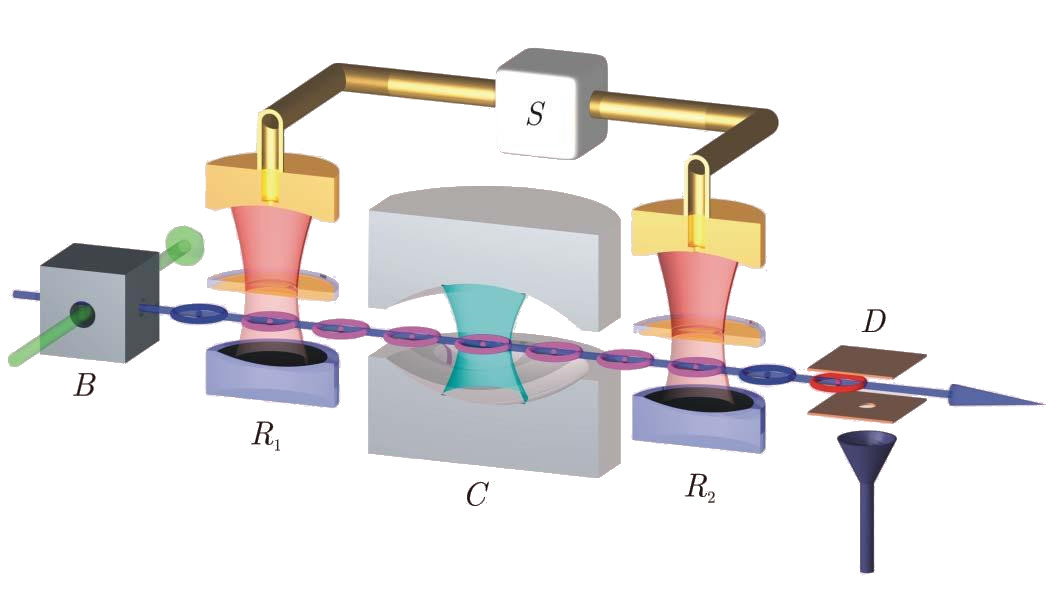
\includegraphics[width=\linewidth]{SH_photon_jumps_setup.jpg}
    \caption{Artist view of the setup used for QND measurement of photons. $B$
    prepares the atoms in a Rydberg state, $R_1$ and $R_2$ both apply a
    $\pi/2$-pulse to the atoms, $D$ uses ionization detection similar to
    Fig.~\ref{fig:ionization_detection}, $C$ is the superconducting cavity,
    cooled down to \SI{0.8}{\kelvin} and detuned
    from the atom transition.}
    \label{fig:QND_setup}
  \end{subfigure}
  ~
  \begin{subfigure}[t]{.48\linewidth}
    \centering
    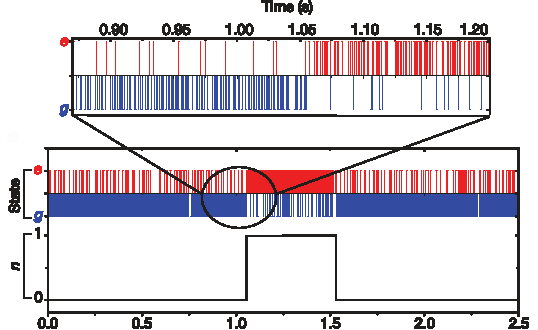
\includegraphics[width=\linewidth]{SH_photon_quantum_jumps_results.pdf}
    \caption{Experimental results of the thermal photon detection. The upper
    trace shows whether the atom was detected in excited (red) or ground (blue)
  state. The lower trace shows the result of a majority vote, decreasing
statistical error and fluctuations. A single photon was first detected at $t_0
\approx$ \SI{1.05}{\second} and observed by several hundreds of atoms during
$\tau \approx \SI{0.5}{\second}$.}
  \label{fig:quantum_jumps_results}
  \end{subfigure}
  \caption{Experimental setup and results of the first realization of quantum
  non demolition measurement of photons. (Source: \cite{gleyzes2007quantum})}
\end{figure}
To calculate the exact phase shift, one has to take into account the detuning of
the cavity, the resonant Rabi frequency, the number of photons in the cavity,
the transverse profile of the cavity mode and
the time of flight of the atoms. But the key point is that some of these
parameters, namely the detuning and the time of flight, can be adjusted such
that
$$ \Phi(\Delta, n) = 
\begin{cases}
  0 & \text{for } n=0 \\
  \pi & \text{for } n=1
\end{cases}
$$
which results in the wave function 
$$ \ket{\Psi_{\text{cav}}} = 
\begin{cases}
  \frac{1}{\sqrt{2}} \left(\ket{e} - i\ket{g}\right) & \text{for } n=0\\
  \frac{1}{\sqrt{2}} \left(\ket{e} + i\ket{g}\right) & \text{for } n=1\\
\end{cases}
$$
At $R_2$ the atoms will receive another $\pi/2$-pulse which, again following
Fig.~\ref{fig:rabi_cycle_rep}, will transform the
wave function to 
$$ \ket{\Psi_{R_2}} = 
\begin{cases}
   i\ket{g} & \text{for } n=0\\
  -\ket{e}  & \text{for } n=1\\
\end{cases}
$$
So by detecting in which Rydberg state the atoms are at $D$, one obtains
information if there are 0 or 1 photons in the cavity. Note that the global
phase of the wave function does not play a role in any physical measurement. The
photon however was not absorbed by the atom, due to the far off detuning of the
cavity and can be detected by the following atom as well until it changes its
state again caused by external perturbation.

One resulting observed pattern is shown in Fig.~\ref{fig:quantum_jumps_results}.
Fluctuations that appear due to statistical uncertainties of the detection
scheme are taken care of by plotting the majority vote, that means the
classification of each event $n$ is based on the results of $n$ and the seven
preceeding events. The shown trace thus shows a photon appearing due to
fluctuations between thermal states and surviving in the cavity for
approximately half a second, corresponding to a traveled distance of light of around
\SI{150000}{\kilo\meter} folded in the cavity.

Haroche and his group found many other applications of this or similar setups,
like engineering multi particle entanglement \cite{rauschenbeutel2000step} and
Schrödinger cat states \cite{brune1992manipulation} or observing
the time evolution of photon number states in a cavity
\cite{guerlin2007progressive}. One could in principle
dive arbitrarly deep into the principles of quantum optics just with the
experiments of Serge Haroche at hand, but this would go far beyond the scope of
this termpaper\footnote{...and the time available to the author.}. Summarizing his work from a current perspective, it shows an
impressive continuity and coherence and definitely deserves\footnote{The author
is aware of the fact that this judgement is not up to him, but anyways...} a Nobel prize as it
tackled numerous fundamental topics of quantum mechanics and quantum
electrodynamics.
